\documentclass[10pt]{beamer}
\usetheme[progressbar=frametitle]{metropolis}
\usepackage{appendixnumberbeamer}
\usepackage[utf8]{inputenc}
\usepackage[backend=bibtex,style=authoryear,doi=false,maxcitenames=1,natbib]{biblatex}
\bibliography{ref.bib}

\usepackage{array,booktabs}
\usepackage[scale=2]{ccicons}
\usepackage{multicol}
\usepackage{mathtools}
\usepackage{array}
\usepackage{colortbl}

\usepackage{pgfplots}
\usepgfplotslibrary{dateplot}
\usepackage{tikz}
\usetikzlibrary{positioning, fit, calc, arrows, decorations.markings}

\usepackage{xspace}
\newcommand{\themename}{\textbf{\textsc{metropolis}}\xspace}
\let\oldfootnotesize\footnotesize
\renewcommand*{\footnotesize}{\oldfootnotesize\tiny}
\let\oldabs\abs
\def\abs{\@ifstar{\oldabs}{\oldabs*}}

\newcolumntype{M}{>{\centering\arraybackslash}p{0.9cm}}
\usepackage{pifont}
\newcommand{\cmark}{\ding{51}}

\usepackage{xcolor}

\newcommand{\cbox}[1]{\raisebox{\depth}{\fcolorbox{black}{#1}{\null}}}

\newcolumntype{Z}{>{\centering\arraybackslash}p{0.9cm}}
\newcolumntype{T}{>{\centering\arraybackslash}p{1.2cm}}

\setbeamerfont{title}{size=\large}
\title{Bringing replication and reproduction together with generalisability in
NLP: Three reproduction studies for Target Dependent Sentiment
Analysis}
\author{Andrew Moore and Paul Rayson}
\date{August 21, 2018}
\institute{School of Computing and Communications, Lancaster University, Lancaster, UK}
\titlegraphic{\hfill
\includegraphics[height=1.5cm]{ucrel_logo_2016.png}}

\newenvironment{packed_enum}{
\begin{enumerate}
  \setlength{\itemsep}{20pt}
  \setlength{\parskip}{0pt}
  \setlength{\parsep}{0pt}
}{\end{enumerate}}

\begin{document}

\maketitle

\begin{frame}{Document Sentiment Example}
\centering
    
    `Rude service, medicore food...there are tons of restaurants in NY...stay away from this one'
    \citep{pontiki_2015}\\
    \textcolor{red}{Negative}

\end{frame}

\begin{frame}{Aspect Based Sentiment Analysis (ABSA) Example}
\centering
\begin{block}{Text}
    `Rude service, medicore food...there are tons of restaurants in NY...stay away from this one'
    \citep{pontiki_2015}
\end{block}
\begin{block}{Aspects}
    \begin{enumerate}
        \item \textcolor{red}{SERVICE\#GENERAL} -- Negative
        \item \textcolor{blue}{FOOD\#QUALITY} -- Neutral
        \item \textcolor{red}{RESTAURANT\#GENERAL} -- Negative
    \end{enumerate}
\end{block}
\end{frame}

\begin{frame}{Target Dependent Sentiment Analysis (TDSA) Example}
\centering
\begin{block}{Text}
    `Rude \textcolor{red}{service}, medicore \textcolor{blue}{food}...there are tons of restaurants in NY...stay away from this one'
    \citep{pontiki_2015}
\end{block}
\begin{block}{Targets}
    \begin{enumerate}
        \item \textcolor{red}{service} -- Negative
        \item \textcolor{blue}{food} -- Neutral
    \end{enumerate}
\end{block}
\end{frame}


\begin{frame}{Generalisability?}

\begin{packed_enum}
    \item Domain -- Restaurant, Laptop
    \item Type -- Social Media, Reviews
    \item Medium -- Written, Spoken
    \item Data Set Size
    \item Data Set Characteristics -- number of targets in a sentence.
\end{packed_enum}

\end{frame}


\begin{frame}{Generalisability within TDSA}
    \begin{table}[!h]
        \centering
        \scalebox{0.7}{
    \begin{tabular}{|l|M|M|M|M|>{\columncolor{gray}}M|>{\columncolor{gray}}M|>{\columncolor{gray}}M|}
            \hline
            &  \multicolumn{7}{c|}{Datasets}  \\
            \hline
            Methods & 1 & 2 & 3 & 4 & \cellcolor{white}{5} & \cellcolor{white}{6} & \cellcolor{white}{7}\\
            \hline
            \hline
            \textcite{mitchell_2013} & \cellcolor{gray} &  & \cmark   & \cellcolor{gray} & & &\\
            \hline
            \textcite{kiritchenko_2014} & \cellcolor{gray} &  &  & \cmark &  &  &\\
            \hline
            \textcite{dong_2014} & \cmark &  & & \cellcolor{gray} & & &\\
            \hline
            \textcite{vo_2015} & \cmark & \cmark & \cmark  & & & & \\
            \hline
            \textcite{zhang_2015} & &  & \cmark  & & & &\\
            \hline
            \textcite{zhang_2016} & \cmark & \cmark & \cmark  & & & & \\
            \hline
            \textcite{Tang_2016_tdlstm} & \cmark &   &  & \cmark & & &\\
            \hline
            \textcite{Tang_2016_mem} & & &   & \cmark & & &\\
            \hline
            \textcite{wang_2016} & &  & & \cmark & & &\\
            \hline
            \textcite{chen_2017} & \cmark &  &   & \cmark & \cellcolor{white}{\cmark} & &\\
            \hline
            \textcite{liu_2017} & \cmark & \cmark & \cmark  &  & &  & \\
            \hline
            \textcite{wang_2017} & \cmark & &   &  &  & \cellcolor{white}{\cmark} &\\
            \hline
            \textcite{Marrese_Taylor_2017} & &  & &   \cmark & &  & \cellcolor{white}{\cmark}\\
            \hline
            \hline
            \multicolumn{8}{|p{13.5cm}|}{1=\textcite{dong_2014}, 2=\textcite{wilson_2008}, 3=\textcite{mitchell_2013}, 4=\textcite{pontiki_2014}, 5=\textcite{chen_2017}, 6=\textcite{wang_2017}, 7=\textcite{Marrese_Taylor_2017}}\\
            \hline
        \end{tabular}
        }
        \caption{Methods and Datasets}
        \label{table:methods_datasets}
    \end{table}
\centering
\cbox{gray} Not Applicable
\end{frame}

\begin{frame}{Generalisability within TDSA}
        \begin{table}[!h]
        \centering
        \scalebox{0.7}{
    \begin{tabular}{|l|>{\columncolor{pink}}M|>{\columncolor{green}}M|>{\columncolor{pink}}M|>{\columncolor{yellow}}M|>{\columncolor{gray}}M|>{\columncolor{gray}}M|>{\columncolor{gray}}M|}
            \hline
            &  \multicolumn{7}{c|}{Datasets}  \\
            \hline
            Methods & 1 & 2 & 3 & 4 & \cellcolor{green}{5} & \cellcolor{pink}{6} & \cellcolor{pink}{7}\\
            \hline
            \hline
            \textcite{mitchell_2013} & \cellcolor{gray} &  & \cmark   & \cellcolor{gray} & & &\\
            \hline
            \textcolor{blue}{\textcite{kiritchenko_2014}} & \cellcolor{gray} &  &  & \cmark &  &  &\\
            \hline
            \textcite{dong_2014} & \cmark &  & & \cellcolor{gray} & & &\\
            \hline
            \textcite{vo_2015} & \cmark & \cmark & \cmark  & & & & \\
            \hline
            \textcite{zhang_2015} & &  & \cmark  & & & &\\
            \hline
            \textcite{zhang_2016} & \cmark & \cmark & \cmark  & & & & \\
            \hline
            \textcite{Tang_2016_tdlstm} & \cmark &   &  & \cmark & & &\\
            \hline
            \textcolor{blue}{\textcite{Tang_2016_mem}} & & &   & \cmark & & &\\
            \hline
            \textcolor{blue}{\textcite{wang_2016}} & &  & & \cmark & & &\\
            \hline
            \textcite{chen_2017} & \cmark &  &   & \cmark & \cellcolor{green}{\cmark} & &\\
            \hline
            \textcite{liu_2017} & \cmark & \cmark & \cmark  &  & &  & \\
            \hline
            \textcite{wang_2017} & \cmark & &   &  &  & \cellcolor{pink}{\cmark} &\\
            \hline
            \textcite{Marrese_Taylor_2017} & &  & &   \cmark & &  & \cellcolor{pink}{\cmark}\\
            \hline
            \hline
            \multicolumn{8}{|p{13.5cm}|}{1=\textcite{dong_2014}, 2=\textcite{wilson_2008}, 3=\textcite{mitchell_2013}, 4=\textcite{pontiki_2014}, 5=\textcite{chen_2017}, 6=\textcite{wang_2017}, 7=\textcite{Marrese_Taylor_2017}}\\
            \hline
        \end{tabular}
        }
        \caption{Methods and Datasets}
        \label{table:methods_datasets}
    \end{table}
\centering
\cbox{pink} Social Media\quad
\cbox{yellow} Reviews\quad
\cbox{green} News\quad
\cbox{gray} Not Applicable
\end{frame}


\begin{frame}{Generalisability within TDSA}
        \begin{table}[!h]
        \centering
        \scalebox{0.7}{
    \begin{tabular}{|l|>{\columncolor{pink}}M|>{\columncolor{green}}M|>{\columncolor{pink}}M|>{\columncolor{yellow}}M|>{\columncolor{gray}}M|>{\columncolor{gray}}M|>{\columncolor{gray}}M|}
            \hline
            &  \multicolumn{7}{c|}{Datasets}  \\
            \hline
            Methods & 1 & 2 & 3 & 4 & \cellcolor{green}{5} & \cellcolor{pink}{6} & \cellcolor{pink}{7}\\
            \hline
            \hline
            \textcolor{blue}{\textcite{mitchell_2013}} & \cellcolor{gray} &  & \cmark   & \cellcolor{gray} & & &\\
            \hline
            \textcite{kiritchenko_2014} & \cellcolor{gray} &  &  & \cmark &  &  &\\
            \hline
            \textcolor{blue}{\textcite{dong_2014}} & \cmark &  & & \cellcolor{gray} & & &\\
            \hline
            \textcolor{blue}{\textcite{vo_2015}} & \cmark & \cmark & \cmark  & & & & \\
            \hline
            \textcolor{blue}{\textcite{zhang_2015}} & &  & \cmark  & & & &\\
            \hline
            \textcolor{blue}{\textcite{zhang_2016}} & \cmark & \cmark & \cmark  & & & & \\
            \hline
            \textcite{Tang_2016_tdlstm} & \cmark &   &  & \cmark & & &\\
            \hline
            \textcite{Tang_2016_mem} & & &   & \cmark & & &\\
            \hline
            \textcite{wang_2016} & &  & & \cmark & & &\\
            \hline
            \textcite{chen_2017} & \cmark &  &   & \cmark & \cellcolor{green}{\cmark} & &\\
            \hline
            \textcolor{blue}{\textcite{liu_2017}} & \cmark & \cmark & \cmark  &  & &  & \\
            \hline
            \textcolor{blue}{\textcite{wang_2017}} & \cmark & &   &  &  & \cellcolor{pink}{\cmark} &\\
            \hline
            \textcite{Marrese_Taylor_2017} & &  & &   \cmark & &  & \cellcolor{pink}{\cmark}\\
            \hline
            \hline
            \multicolumn{8}{|p{13.5cm}|}{1=\textcite{dong_2014}, 2=\textcite{wilson_2008}, 3=\textcite{mitchell_2013}, 4=\textcite{pontiki_2014}, 5=\textcite{chen_2017}, 6=\textcite{wang_2017}, 7=\textcite{Marrese_Taylor_2017}}\\
            \hline
        \end{tabular}
        }
        \caption{Methods and Datasets}
        \label{table:methods_datasets}
    \end{table}
\centering
\cbox{pink} Social Media\quad
\cbox{yellow} Reviews\quad
\cbox{green} News\quad
\cbox{gray} Not Applicable
\end{frame}


\begin{frame}{Generalisability within TDSA}
    \begin{table}[!h]
        \centering
        \scalebox{0.7}{
    \begin{tabular}{|l|>{\columncolor{pink}}M|>{\columncolor{green}}M|>{\columncolor{pink}}M|>{\columncolor{yellow}}M|>{\columncolor{gray}}M|>{\columncolor{gray}}M|>{\columncolor{gray}}M|}
            \hline
            &  \multicolumn{7}{c|}{Datasets}  \\
            \hline
            Methods & 1 & 2 & 3 & 4 & \cellcolor{green}{5} & \cellcolor{pink}{6} & \cellcolor{pink}{7}\\
            \hline
            \hline
            \textcite{mitchell_2013} & \cellcolor{gray} &  & \cmark   & \cellcolor{gray} & & &\\
            \hline
            \textcite{kiritchenko_2014} & \cellcolor{gray} &  &  & \cmark &  &  &\\
            \hline
            \textcite{dong_2014} & \cmark &  & & \cellcolor{gray} & & &\\
            \hline
            \textcolor{blue}{\textcite{vo_2015}} & \cmark & \cmark & \cmark  & & & & \\
            \hline
            \textcite{zhang_2015} & &  & \cmark  & & & &\\
            \hline
            \textcite{zhang_2016} & \cmark & \cmark & \cmark  & & & & \\
            \hline
            \textcolor{blue}{\textcite{Tang_2016_tdlstm}} & \cmark &   &  & \cmark & & &\\
            \hline
            \textcite{Tang_2016_mem} & & &   & \cmark & & &\\
            \hline
            \textcite{wang_2016} & &  & & \cmark & & &\\
            \hline
            \textcite{chen_2017} & \cmark &  &   & \cmark & \cellcolor{green}{\cmark} & &\\
            \hline
            \textcite{liu_2017} & \cmark & \cmark & \cmark  &  & &  & \\
            \hline
            \textcolor{blue}{\textcite{wang_2017}} & \cmark & &   &  &  & \cellcolor{pink}{\cmark} &\\
            \hline
            \textcite{Marrese_Taylor_2017} & &  & &   \cmark & &  & \cellcolor{pink}{\cmark}\\
            \hline
            \hline
            \multicolumn{8}{|p{13.5cm}|}{1=\textcite{dong_2014}, 2=\textcite{wilson_2008}, 3=\textcite{mitchell_2013}, 4=\textcite{pontiki_2014}, 5=\textcite{chen_2017}, 6=\textcite{wang_2017}, 7=\textcite{Marrese_Taylor_2017}}\\
            \hline
        \end{tabular}
        }
        \caption{Methods and Datasets}
        \label{table:methods_datasets}
    \end{table}
\centering
\cbox{pink} Social Media\quad
\cbox{yellow} Reviews\quad
\cbox{green} News\quad
\cbox{gray} Not Applicable
\end{frame}

\begin{frame}{Why Reproduce?}
\begin{table}[]
    \centering
    \begin{tabular}{|c|c|}
        \hline
        Authors & Code with paper \\
        \hline
        \textcite{wang_2017} & Yes \\
        \hline
        \textcite{Tang_2016_tdlstm} & Unreliable \\
        \hline
        \textcite{vo_2015} & No \\
        \hline
    \end{tabular}
\end{table}

    \begin{table}[!h]
\centering
\begin{tabular}{|l|c|c|}
\hline
Authors & Restaurant & Laptop \\
\hline
\textcolor{blue}{\textcite{Tang_2016_tdlstm}} & 75.63 & 68.13 \\
\hline
\textcolor{orange}{\textcite{chen_2017}} & 78.00 & 71.83 \\
\hline
\textcolor{red}{\textcite{tay_2017}} & 69.73 & 62.38 \\
\hline
\end{tabular}
\end{table}
\centering
\cbox{blue} Original\quad
\cbox{orange} Re-used the same code\quad
\cbox{red} Re-implemented
\end{frame}


\begin{frame}{\textcite{vo_2015} Method}
\centering
\resizebox{11.0cm}{!}{%
    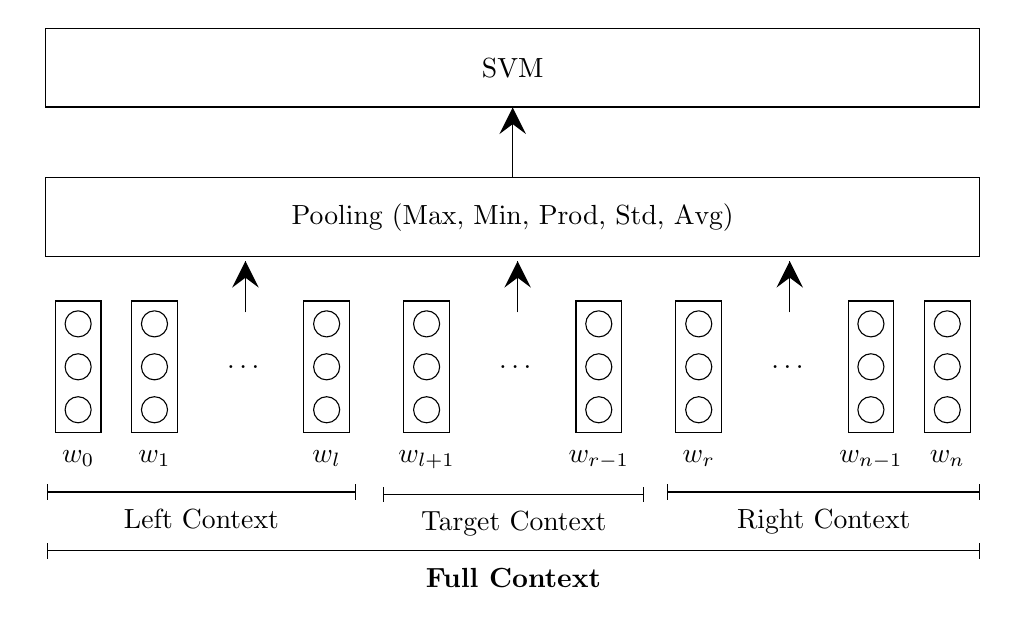
\begin{tikzpicture}[
    feature/.style={circle, draw, radius=0.05},
    vector/.style={rectangle, draw, minimum height=1cm},
    arrow_pointer/.style={decoration={markings,mark=at position 1 with %
    {\arrow[scale=3,>=stealth]{>}}},postaction={decorate}}]
    
    % Left Context
    \node[feature](feat1){};
    \node[feature, below=.2 of feat1](feat2){};
    \node[feature, above=.2 of feat1](feat0){};
	\node[vector, fit=(feat0)(feat1)(feat2)] (vec0) {};
	\node[below=.1 of vec0] (x0) {$w_0$};
	
	\node[feature, right=.5 of vec0](feat4){};
    \node[feature, below=.2 of feat4](feat5){};
    \node[feature, above=.2 of feat4](feat3){};
	\node[vector, fit=(feat4)(feat3)(feat5)] (vec1) {};
	\node[below=.1 of vec1] (x1) {$w_1$};
	
	\node[right=.5 of vec1](dot0){$\dots$};
	
	\node[feature, right=.5of dot0](feat7){};
    \node[feature, below=.2 of feat7](feat8){};
    \node[feature, above=.2 of feat7](feat6){};
	\node[vector, fit=(feat7)(feat6)(feat8)] (vec2) {};
	\node[below=.1 of vec2] (x2) {$w_l$};
	
	\node[below left=.1 of x0] (line0) {};
	\node[below right=.1 of x2] (line1) {};
	\draw [|-|] (line0) -- (line1)  node[pos=0.5, below=0.1]{Left Context};
	
	% Target Context
	\node[feature, right=.8 of vec2](feat10){};
    \node[feature, below=.2 of feat10](feat11){};
    \node[feature, above=.2 of feat10](feat9){};
	\node[vector, fit=(feat10)(feat9)(feat11)] (vec3) {};
	\node[below=.1 of vec3] (x3) {$w_{l+1}$};
	
	\node[right=.5 of vec3](dot1){$\dots$};
	
	\node[feature, right=.5 of dot1](feat13){};
    \node[feature, below=.2 of feat13](feat14){};
    \node[feature, above=.2 of feat13](feat12){};
	\node[vector, fit=(feat13)(feat12)(feat14)] (vec4) {};
	\node[below=.1 of vec4] (x4) {$w_{r-1}$};
	
	\node[below left=.1 of x3] (line2) {};
	\node[below right=.1 of x4] (line3) {};
	\draw [|-|] (line2) -- (line3)  node[pos=0.5, below=0.1]{Target Context};
	
	% Right Context
	\node[feature, right=.8 of vec4](feat16){};
    \node[feature, below=.2 of feat16](feat17){};
    \node[feature, above=.2 of feat16](feat15){};
	\node[vector, fit=(feat16)(feat15)(feat17)] (vec5) {};
	\node[below=.1 of vec5] (x5) {$w_r$};
	
	\node[right=.5 of vec5](dot2){$\dots$};
	
	\node[feature, right=.5 of dot2](feat19){};
    \node[feature, below=.2 of feat19](feat20){};
    \node[feature, above=.2 of feat19](feat18){};
	\node[vector, fit=(feat19)(feat18)(feat20)] (vec6) {};
	\node[below=.1 of vec6] (x6) {$w_{n-1}$};
	
	\node[feature, right=.5 of vec6](feat22){};
    \node[feature, below=.2 of feat22](feat23){};
    \node[feature, above=.2 of feat22](feat21){};
	\node[vector, fit=(feat22)(feat21)(feat23)] (vec7) {};
	\node[below=.1 of vec7] (x7) {$w_n$};
	
	\node[below left=.1 of x5] (line4) {};
	\node[below right=.1 of x7] (line5) {};
	\draw [|-|] (line4) -- (line5)  node[pos=0.5, below=0.1]{Right Context};
	
	\node[below=.5 of line0] (line6) {};
	\node[below=.5 of line5] (line7) {};
	\draw [|-|] (line6) -- (line7)  node[pos=0.5, below=0.1]{\textbf{Full Context}};
	
	\node[rectangle, draw, minimum width=3em, above=1.9, fit={(vec0.west) (vec7.east)}, minimum height = 1cm, inner ysep=0pt, label={center:Pooling (Max, Min, Prod, Std, Avg)}] (pooling) {};
	
	% Arrows for the context to the pooling layer
	% Left context
	\node[above=.3 of dot0] (top_dot0) {};
	\node[above=1.2 of dot0] (top_top_dot0) {};
	\draw [arrow_pointer] (top_dot0) -- (top_top_dot0);
	
	% Center context
	\node[above=.3 of dot1] (top_dot1) {};
	\node[above=1.2 of dot1] (top_top_dot1) {};
	\draw [arrow_pointer] (top_dot1) -- (top_top_dot1);
	
	% Right context
	\node[above=.3 of dot2] (top_dot2) {};
	\node[above=1.2 of dot2] (top_top_dot2) {};
	\draw [arrow_pointer] (top_dot2) -- (top_top_dot2);
	
	\node[rectangle, draw, minimum width=3em, above=3.8, fit={(vec0.west) (vec7.east)}, minimum height = 1cm, inner ysep=0pt, label={center:SVM}] (svm) {};
	\draw [arrow_pointer] (pooling) -- (svm);
\label{fig:vo_method}
\end{tikzpicture}}
\end{frame}

\begin{frame}{\textcite{vo_2015} Reproduction Result}
\centering
    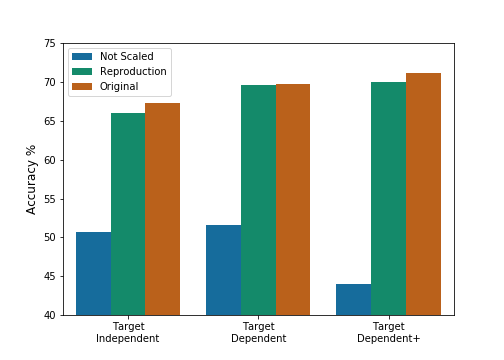
\includegraphics[scale=0.55]{Target_Results.png}
    %\includegraphics[scale=0.55]{Target_Results_old.png}
    \\\textbf{Scaling features is important - 15-25\% difference}
\end{frame}

%\begin{frame}{\textcite{wang_2017} Method}
%\centering
%    \resizebox{11.0cm}{!}{%
%    \begin{tikzpicture}[
%    feature/.style={circle, draw, radius=0.05},
%    vector/.style={rectangle, draw, minimum height=1cm},
%    arrow_pointer/.style={decoration={markings,mark=at position 1 with %
%    {\arrow[scale=3,>=stealth]{>}}},postaction={decorate}}]
    
    % Left Context
%    \node[feature](feat1){};
%    \node[feature, below=.2 of feat1](feat2){};
%    \node[feature, above=.2 of feat1](feat0){};
%	\node[vector, fit=(feat0)(feat1)(feat2)] (vec0) {};
%	\node[below=.1 of vec0] (x0) {$w_0$};
	
%	\node[feature, right=.5 of vec0](feat4){};
%    \node[feature, below=.2 of feat4](feat5){};
%    \node[feature, above=.2 of feat4](feat3){};
%	\node[vector, fit=(feat4)(feat3)(feat5)] (vec1) {};
%	\node[below=.1 of vec1] (x1) {$w_1$};
	
%	\node[right=.5 of vec1](dot0){$\dots$};
	
%	\node[feature, right=.5of dot0](feat7){};
%   \node[feature, below=.2 of feat7](feat8){};
%    \node[feature, above=.2 of feat7](feat6){};
%	\node[vector, fit=(feat7)(feat6)(feat8)] (vec2) {};
%	\node[below=.1 of vec2] (x2) {$w_l$};
	
%	\node[below left=.1 of x0] (line0) {};
%	\node[below right=.1 of x2] (line1) {};
%	\draw [|-|] (line0) -- (line1)  node[pos=0.5, below=0.1]{Left Context};
	
	% Target Context
%	\node[feature, right=.8 of vec2](feat10){};
%    \node[feature, below=.2 of feat10](feat11){};
%    \node[feature, above=.2 of feat10](feat9){};
%	\node[vector, fit=(feat10)(feat9)(feat11)] (vec3) {};
%	\node[below=.1 of vec3] (x3) {$w_{l+1}$};
	
%	\node[right=.5 of vec3](dot1){$\dots$};
	
%	\node[feature, right=.5 of dot1](feat13){};
%    \node[feature, below=.2 of feat13](feat14){};
%    \node[feature, above=.2 of feat13](feat12){};
%	\node[vector, fit=(feat13)(feat12)(feat14)] (vec4) {};
%	\node[below=.1 of vec4] (x4) {$w_{r-1}$};
	
%	\node[below left=.1 of x3] (line2) {};
%	\node[below right=.1 of x4] (line3) {};
%	\draw [|-|] (line2) -- (line3)  node[pos=0.5, below=0.1]{Target Context};
	
	% Right Context
%	\node[feature, right=.8 of vec4](feat16){};
%    \node[feature, below=.2 of feat16](feat17){};
%    \node[feature, above=.2 of feat16](feat15){};
%	\node[vector, fit=(feat16)(feat15)(feat17)] (vec5) {};
%	\node[below=.1 of vec5] (x5) {$w_r$};
	
%	\node[right=.5 of vec5](dot2){$\dots$};
	
%	\node[feature, right=.5 of dot2](feat19){};
%    \node[feature, below=.2 of feat19](feat20){};
%    \node[feature, above=.2 of feat19](feat18){};
%	\node[vector, fit=(feat19)(feat18)(feat20)] (vec6) {};
%	\node[below=.1 of vec6] (x6) {$w_{n-1}$};
	
%	\node[feature, right=.5 of vec6](feat22){};
%    \node[feature, below=.2 of feat22](feat23){};
%    \node[feature, above=.2 of feat22](feat21){};
%	\node[vector, fit=(feat22)(feat21)(feat23)] (vec7) {};
%	\node[below=.1 of vec7] (x7) {$w_n$};
	
%	\node[below left=.1 of x5] (line4) {};
%	\node[below right=.1 of x7] (line5) {};
%	\draw [|-|] (line4) -- (line5)  node[pos=0.5, below=0.1]{Right Context};
	
%	\node[below=.5 of line0] (line6) {};
%	\node[below=.5 of line5] (line7) {};
%	\draw [|-|] (line6) -- (line7)  node[pos=0.5, below=0.1]{\textbf{Dependency Context}};
	
%	\node[rectangle, draw, minimum width=3em, above=1.9, fit={(vec0.west) (vec7.east)}, minimum height = 1cm, inner ysep=0pt, label={center:Pooling (Max, Min, Prod, Std, Avg)}] (pooling) {};
	
	% Arrows for the context to the pooling layer
	% Left context
%	\node[above=.3 of dot0] (top_dot0) {};
%	\node[above=1.2 of dot0] (top_top_dot0) {};
%	\draw [arrow_pointer] (top_dot0) -- (top_top_dot0);
	
	% Center context
%	\node[above=.3 of dot1] (top_dot1) {};
%	\node[above=1.2 of dot1] (top_top_dot1) {};
%	\draw [arrow_pointer] (top_dot1) -- (top_top_dot1);
	
	% Right context
%	\node[above=.3 of dot2] (top_dot2) {};
%	\node[above=1.2 of dot2] (top_top_dot2) {};
%	\draw [arrow_pointer] (top_dot2) -- (top_top_dot2);
	
%	\node[rectangle, draw, minimum width=3em, above=3.8, fit={(vec0.west) (vec7.east)}, minimum height = 1cm, inner ysep=0pt, label={center:SVM}] (svm) {};
%	\draw [arrow_pointer] (pooling) -- (svm);
%\label{fig:wang_method}
%\end{tikzpicture}}
%\end{frame}

%\begin{frame}{\textcite{wang_2017} Replication Result}
%    \includegraphics[scale=0.55]{TDParse_Results.png}
%\end{frame}

\begin{frame}{\textcite{Tang_2016_tdlstm} Method}
    \centering
    \resizebox{11.0cm}{!}{%
    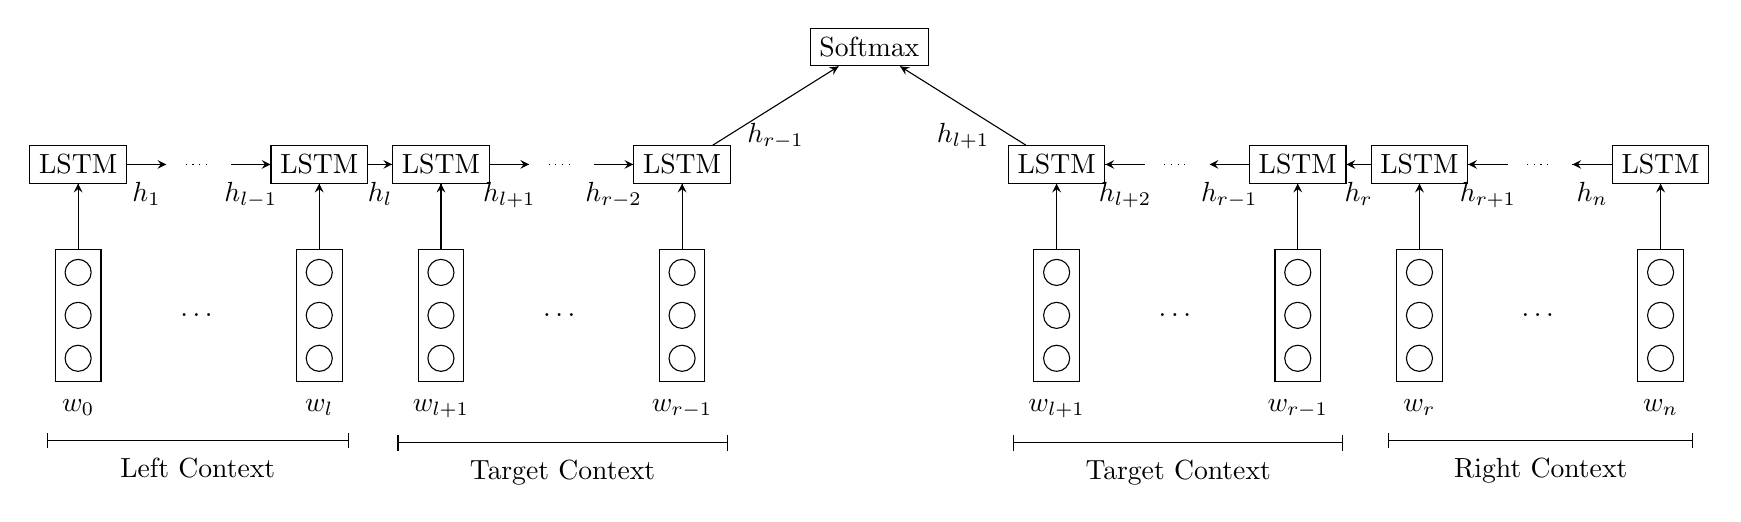
\begin{tikzpicture}[
    feature/.style={circle, draw, radius=0.05},
    vector/.style={rectangle, draw, minimum height=1cm},
    lstm_node/.style={rectangle, draw},
    arrow_pointer/.style={decoration={markings,mark=at position 1 with %
    {\arrow[scale=1,>=stealth]{>}}},postaction={decorate}}]
    
    % Left Context
    \node[feature](feat1){};
    \node[feature, below=.2 of feat1](feat2){};
    \node[feature, above=.2 of feat1](feat0){};
	\node[vector, fit=(feat0)(feat1)(feat2)] (vec0) {};
	\node[below=.1 of vec0] (x0) {$w_0$};
	% LSTM 0
	\node[lstm_node, above=1.5 of feat1](lstm0){LSTM};
	\draw [arrow_pointer] (vec0) -- (lstm0);
	
	\node[right=1 of feat1](dot0){$\dots$};
	
	\node[feature, right=1 of dot0](feat4){};
    \node[feature, below=.2 of feat4](feat5){};
    \node[feature, above=.2 of feat4](feat3){};
	\node[vector, fit=(feat4)(feat3)(feat5)] (vec1) {};
	\node[below=.1 of vec1] (x1) {$w_l$};
	% LSTM 1
	\node[lstm_node, above=1.5 of feat4](lstm1){LSTM};
	\draw [arrow_pointer] (vec1) -- (lstm1);
	
	% Arrows between LSTMs
	\node[right=.5 of lstm0] (lstm0_left_mid) {};
	\node[left=.5 of lstm1] (lstm0_right_mid) {};
	\draw [arrow_pointer] (lstm0) -- (lstm0_left_mid) node[pos=0.5, below=0.1]{$h_1$};
	\draw[dotted](lstm0_left_mid) -- (lstm0_right_mid);
	\draw [arrow_pointer] (lstm0_right_mid) -- (lstm1) node[pos=0.5, below=0.1]{$h_{l-1}$};
	
	
	
	\node[feature, right=1.2 of feat4](feat7){};
    \node[feature, below=.2 of feat7](feat8){};
    \node[feature, above=.2 of feat7](feat6){};
	\node[vector, fit=(feat7)(feat6)(feat8)] (vec2) {};
	\node[below=.1 of vec2] (x2) {$w_{l+1}$};
	
	\node[right=1 of feat7](dot1){$\dots$};
	% LSTM 2
	\node[lstm_node, above=1.5 of feat7](lstm2){LSTM};
	\draw [arrow_pointer] (vec2) -- (lstm2);
	\draw [arrow_pointer] (lstm1) -- (lstm2) node[pos=0.5, below=0.1]{$h_l$};
	
	\node[feature, right=1 of dot1](feat10){};
    \node[feature, below=.2 of feat10](feat11){};
    \node[feature, above=.2 of feat10](feat9){};
	\node[vector, fit=(feat10)(feat9)(feat11)] (vec3) {};
	\node[below=.1 of vec3] (x3) {$w_{r-1}$};
	% LSTM 3
	\node[lstm_node, above=1.5 of feat10](lstm3){LSTM};
	\draw [arrow_pointer] (vec3) -- (lstm3);
	
	% Arrows between LSTMs
	\node[right=.5 of lstm2] (lstm2_left_mid) {};
	\node[left=.5 of lstm3] (lstm2_right_mid) {};
	\draw [arrow_pointer] (lstm2) -- (lstm2_left_mid) node[pos=0.5, below=0.1]{$h_{l+1}$};
	\draw[dotted](lstm2_left_mid) -- (lstm2_right_mid);
	\draw [arrow_pointer] (lstm2_right_mid) -- (lstm3) node[pos=0.5, below=0.1]{$h_{r-2}$};
	
	% Softmax
	\node[rectangle, draw, above right= of lstm3] (softmax) {Softmax};
	\draw [arrow_pointer] (lstm3) -- (softmax) node[pos=0.5, below=0.1]{$h_{r-1}$};
	
	
	% Right Context
	\node[lstm_node, below right=of softmax](lstm4){LSTM};
	\draw [arrow_pointer] (lstm4) -- (softmax) node[pos=0.5, below=0.1]{$h_{l+1}$};
	
    \node[feature, below=1.5 of lstm4](feat13){};
    \node[feature, below=.2 of feat13](feat14){};
    \node[feature, above=.2 of feat13](feat12){};
	\node[vector, fit=(feat12)(feat13)(feat14)] (vec4) {};
	\node[below=.1 of vec4] (x4) {$w_{l+1}$};
	\draw [arrow_pointer] (vec4) -- (lstm4);
	
	\node[right=1 of feat13](dot2){$\dots$};
	
    \node[feature, right=of dot2](feat16){};
    \node[feature, below=.2 of feat16](feat17){};
    \node[feature, above=.2 of feat16](feat15){};
	\node[vector, fit=(feat15)(feat16)(feat17)] (vec5) {};
	\node[below=.1 of vec5] (x5) {$w_{r-1}$};
	% LSTM 5
	\node[lstm_node, above=1.5 of feat16](lstm5){LSTM};
	\draw [arrow_pointer] (vec5) -- (lstm5);
	
	% Arrows between LSTMs
	\node[right=.5 of lstm4] (lstm4_left_mid) {};
	\node[left=.5 of lstm5] (lstm4_right_mid) {};
	\draw [arrow_pointer] (lstm4_left_mid) -- (lstm4) node[pos=0.5, below=0.1]{$h_{l+2}$};
	\draw[dotted](lstm4_left_mid) -- (lstm4_right_mid);
	\draw [arrow_pointer] (lstm5) -- (lstm4_right_mid) node[pos=0.5, below=0.1]{$h_{r-1}$};
	
	\node[feature, right=1.2 of feat16](feat19){};
    \node[feature, below=.2 of feat19](feat20){};
    \node[feature, above=.2 of feat19](feat18){};
	\node[vector, fit=(feat18)(feat19)(feat20)] (vec6) {};
	\node[below=.1 of vec6] (x6) {$w_r$};
	% LSTM 6
	\node[lstm_node, above=1.5 of feat19](lstm6){LSTM};
	\draw [arrow_pointer] (vec6) -- (lstm6);
	\draw [arrow_pointer] (lstm6) -- (lstm5) node[pos=0.5, below=0.1]{$h_r$};
	
	\node[right=1 of feat19](dot3){$\dots$};
	
	\node[feature, right=of dot3](feat22){};
    \node[feature, below=.2 of feat22](feat23){};
    \node[feature, above=.2 of feat22](feat21){};
	\node[vector, fit=(feat21)(feat22)(feat23)] (vec7) {};
	\node[below=.1 of vec7] (x7) {$w_n$};
	% LSTM 7
	\node[lstm_node, above=1.5 of feat22](lstm7){LSTM};
	\draw [arrow_pointer] (vec7) -- (lstm7);
	
	% Arrows between LSTMs
	\node[right=.5 of lstm6] (lstm6_left_mid) {};
	\node[left=.5 of lstm7] (lstm6_right_mid) {};
	\draw [arrow_pointer] (lstm6_left_mid) -- (lstm6) node[pos=0.5, below=0.1]{$h_{r+1}$};
	\draw[dotted](lstm6_left_mid) -- (lstm6_right_mid);
	\draw [arrow_pointer] (lstm7) -- (lstm6_right_mid) node[pos=0.5, below=0.1]{$h_n$};
	
	% Left context arrows
	\node[below left=.1 of x0] (line0) {};
	\node[below right=.1 of x1] (line1) {};
	\draw [|-|] (line0) -- (line1)  node[pos=0.5, below=0.1]{Left Context};
	
	% Left Target context arrows
	\node[below left=.1 of x2] (line2) {};
	\node[below right=.1 of x3] (line3) {};
	\draw [|-|] (line2) -- (line3)  node[pos=0.5, below=0.1]{Target Context};
	
	% Right Target context arrows
	\node[below left=.1 of x4] (line4) {};
	\node[below right=.1 of x5] (line5) {};
	\draw [|-|] (line4) -- (line5)  node[pos=0.5, below=0.1]{Target Context};
	
	% Right context arrows
	\node[below left=.1 of x6] (line6) {};
	\node[below right=.1 of x7] (line7) {};
	\draw [|-|] (line6) -- (line7)  node[pos=0.5, below=0.1]{Right Context};
	

	
	
\label{fig:wang_method}
\end{tikzpicture}}
\end{frame}

\begin{frame}{\textcite{Tang_2016_tdlstm} Reproduction Result}

\begin{columns}[T,onlytextwidth]
    \column{0.48\textwidth}
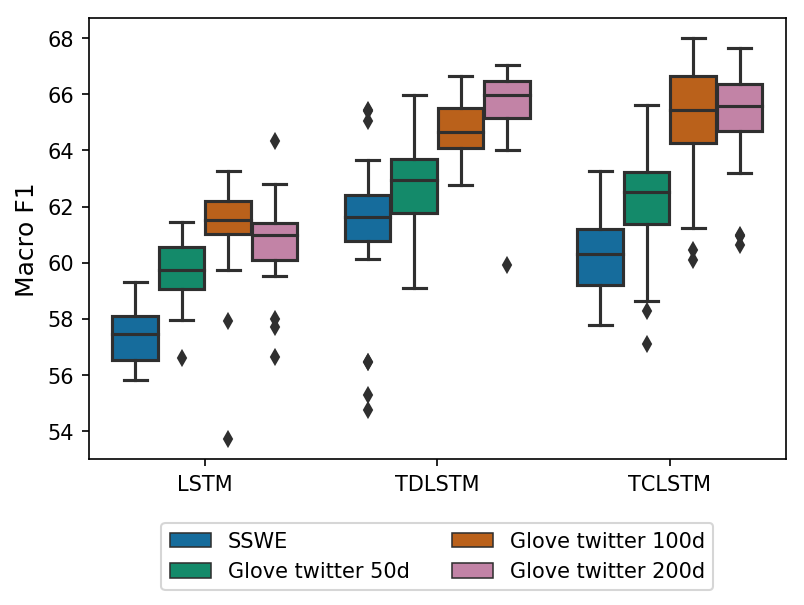
\includegraphics[scale=0.4]{TDLSTM_Word_Embeddings_Color.png}
\column{0.48\textwidth}
 \resizebox{6.0cm}{!}{%
\begin{tabular}{|l|c|c|c|}
\hline
 & \multicolumn{3}{c|}{Macro F1} \\
\hline
Methods& O & R (Max) & R (Mean) \\
\hline
\hline
LSTM & 64.70 & 64.34 & 60.69 \\
\hline
TDLSTM & 69.00 & 67.04 & 65.63\\
\hline
TCLSTM & 69.50 & 67.66 & 65.23\\
\hline
\hline
\multicolumn{4}{|c|}{O=Original, R=Reproduction}\\
\hline
\end{tabular}
}
\end{columns}
\vspace{1cm}
\textbf{Repeating experiments with different seed values is important. \citep{reimers2017reporting}}
\end{frame}

\begin{frame}{Mass Evaluation Datasets}
\centering
    \begin{tabular}{|c|c|c|c|c|c|}
            \hline
            Dataset & Domain & Type & Size & Medium & ATS\\
            \hline
            \hline
            SemEval 14 L& L & RE & 2951 & W & 1.58 \\
            \hline
            SemEval 14 R& R & RE & 4722 & W & 1.83 \\
            \hline
            Mitchel & G & S & 3288 & W & 1.22  \\
            \hline
        Dong Twitter& G & S & 6940 & W & 1.00 \\
            \hline
            Election Twitter& P & S & 11899 & W & 2.94 \\
            \hline
            YouTuBean& MP & RE/S& 798 & SP & 2.07 \\
            \hline
            \hline
            \multicolumn{6}{|p{\linewidth}|}{L=Laptop, R=Restaurant, G=General, P=Politics, MP=Mobile Phones, RE=Review, S=Social Media, W=Written, SP=Spoken, ATS=Average Targets per Sentence}\\
            \hline
        \end{tabular}
\end{frame}

\begin{frame}{Mass Evaluation}
\centering
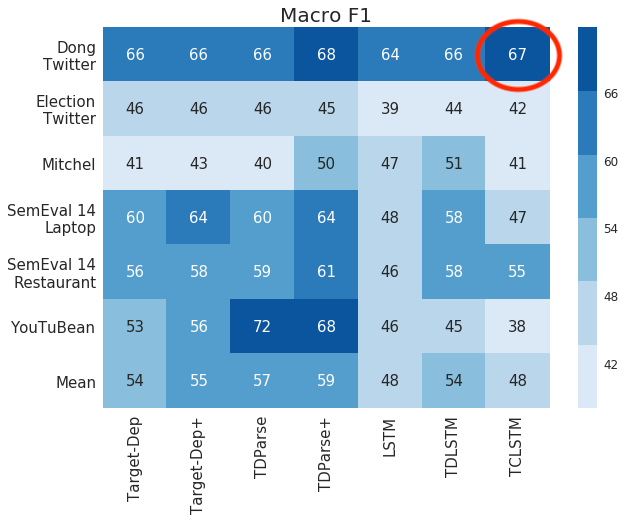
\includegraphics[scale=0.45]{mass_eval1.png}
\end{frame}

\begin{frame}{Mass Evaluation}
\centering
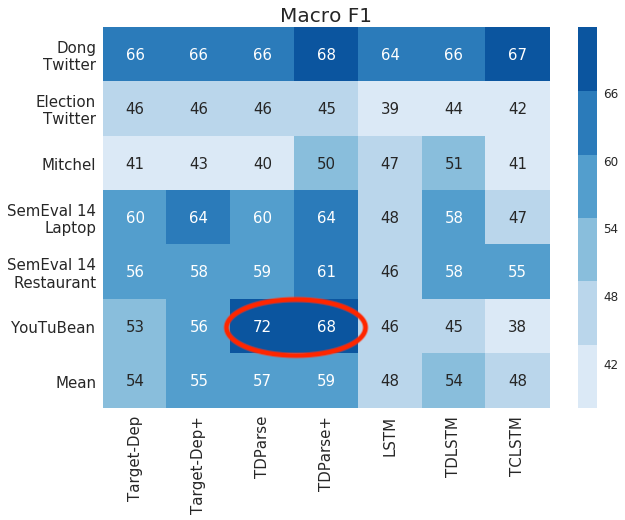
\includegraphics[scale=0.45]{mass_eval2.png}
\end{frame}

%\begin{frame}{Mass Evaluation}
%\centering
%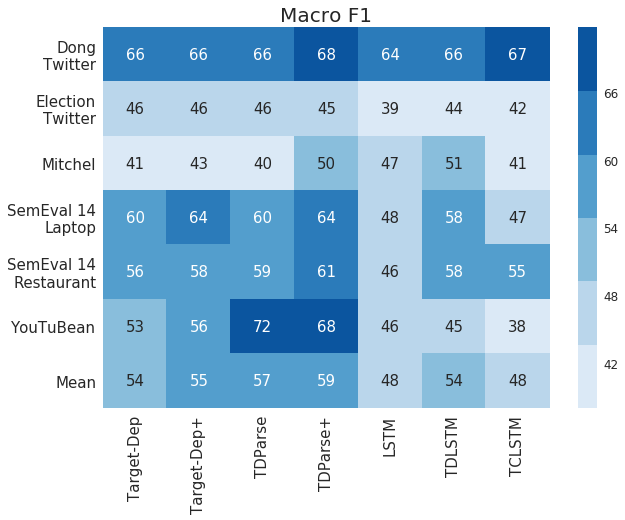
\includegraphics[scale=0.45]{mass_eval.png}
%\end{frame}

\begin{frame}[t]{Contributions}
\vspace{1cm}
\centering
    \begin{packed_enum}
        \item \textbf{Generalisability}: First to report results across across three different dataset properties: 1. Domain, 2. Type, 3. Medium.
        %Report results on all possible datasets. Not selected datasets.
        \item \textbf{Reproduction}: Open source TDSA framework with three different models.
        %Deep Learning methods require more than single run results.\citep{reimers2017reporting}
        %\item Where possible release \textbf{code} and \textbf{data}
    \end{packed_enum}
    \vspace{10pt}
    Code, documentation, Jupyter notebook examples, and model zoo:
    \url{https://github.com/apmoore1/Bella}\\
    \vspace{10pt}
    a.moore@lancaster.ac.uk\\
    @apmoore94 and @perayson
\end{frame}



%\appendix
\begin{frame}[noframenumbering,plain,allowframebreaks]{References}
  \printbibliography[heading=none]
\end{frame}

\end{document}

